\documentclass[]{article}
\usepackage{lmodern}
\usepackage{amssymb,amsmath}
\usepackage{ifxetex,ifluatex}
\usepackage{fixltx2e} % provides \textsubscript
\ifnum 0\ifxetex 1\fi\ifluatex 1\fi=0 % if pdftex
  \usepackage[T1]{fontenc}
  \usepackage[utf8]{inputenc}
\else % if luatex or xelatex
  \ifxetex
    \usepackage{mathspec}
  \else
    \usepackage{fontspec}
  \fi
  \defaultfontfeatures{Ligatures=TeX,Scale=MatchLowercase}
\fi
% use upquote if available, for straight quotes in verbatim environments
\IfFileExists{upquote.sty}{\usepackage{upquote}}{}
% use microtype if available
\IfFileExists{microtype.sty}{%
\usepackage{microtype}
\UseMicrotypeSet[protrusion]{basicmath} % disable protrusion for tt fonts
}{}
\usepackage[margin=1in]{geometry}
\usepackage{hyperref}
\hypersetup{unicode=true,
            pdftitle={Effectiveness of community-based marine reserves in small-scale fisheries},
            pdfborder={0 0 0},
            breaklinks=true}
\urlstyle{same}  % don't use monospace font for urls
\usepackage{longtable,booktabs}
\usepackage{graphicx,grffile}
\makeatletter
\def\maxwidth{\ifdim\Gin@nat@width>\linewidth\linewidth\else\Gin@nat@width\fi}
\def\maxheight{\ifdim\Gin@nat@height>\textheight\textheight\else\Gin@nat@height\fi}
\makeatother
% Scale images if necessary, so that they will not overflow the page
% margins by default, and it is still possible to overwrite the defaults
% using explicit options in \includegraphics[width, height, ...]{}
\setkeys{Gin}{width=\maxwidth,height=\maxheight,keepaspectratio}
\IfFileExists{parskip.sty}{%
\usepackage{parskip}
}{% else
\setlength{\parindent}{0pt}
\setlength{\parskip}{6pt plus 2pt minus 1pt}
}
\setlength{\emergencystretch}{3em}  % prevent overfull lines
\providecommand{\tightlist}{%
  \setlength{\itemsep}{0pt}\setlength{\parskip}{0pt}}
\setcounter{secnumdepth}{5}
% Redefines (sub)paragraphs to behave more like sections
\ifx\paragraph\undefined\else
\let\oldparagraph\paragraph
\renewcommand{\paragraph}[1]{\oldparagraph{#1}\mbox{}}
\fi
\ifx\subparagraph\undefined\else
\let\oldsubparagraph\subparagraph
\renewcommand{\subparagraph}[1]{\oldsubparagraph{#1}\mbox{}}
\fi

%%% Use protect on footnotes to avoid problems with footnotes in titles
\let\rmarkdownfootnote\footnote%
\def\footnote{\protect\rmarkdownfootnote}

%%% Change title format to be more compact
\usepackage{titling}

% Create subtitle command for use in maketitle
\newcommand{\subtitle}[1]{
  \posttitle{
    \begin{center}\large#1\end{center}
    }
}

\setlength{\droptitle}{-2em}

  \title{Effectiveness of community-based marine reserves in small-scale
fisheries}
    \pretitle{\vspace{\droptitle}\centering\huge}
  \posttitle{\par}
    \author{}
    \preauthor{}\postauthor{}
    \date{}
    \predate{}\postdate{}
  

\begin{document}
\maketitle

{
\setcounter{tocdepth}{2}
\tableofcontents
}
\hypertarget{data}{%
\section{Data}\label{data}}

\begin{table}

\caption{\label{tab:unnamed-chunk-2}Number of invertebrate transects performed in each site of each community.}
\centering
\begin{tabular}[t]{l|r|r}
\hline
Community & Control & Reserve\\
\hline
Isla Natividad & 415 & 244\\
\hline
Maria Elena & 27 & 21\\
\hline
Punta Herrero & 51 & 73\\
\hline
\end{tabular}
\end{table}

\includegraphics{SupplementaryMaterial_files/figure-latex/unnamed-chunk-3-1.pdf}

\includegraphics{SupplementaryMaterial_files/figure-latex/unnamed-chunk-4-1.pdf}

\begin{table}

\caption{\label{tab:unnamed-chunk-5}Number of fish transects performed in each site of each community.}
\centering
\begin{tabular}[t]{l|r|r}
\hline
Community & Control & Reserve\\
\hline
Isla Natividad & 400 & 240\\
\hline
Maria Elena & 44 & 45\\
\hline
Punta Herrero & 82 & 85\\
\hline
\end{tabular}
\end{table}

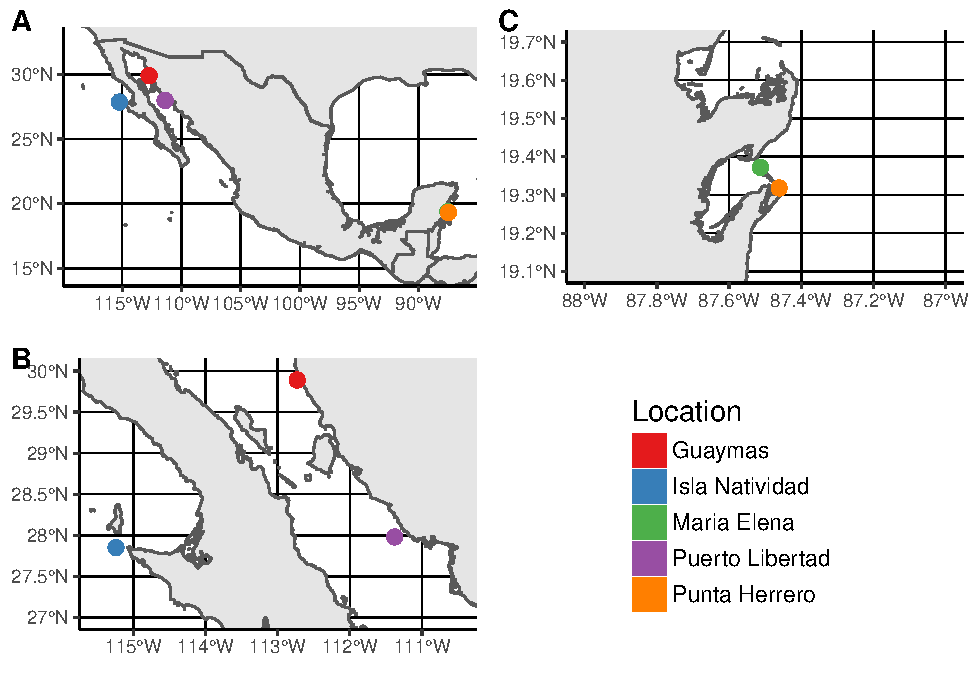
\includegraphics{SupplementaryMaterial_files/figure-latex/unnamed-chunk-6-1.pdf}

\includegraphics{SupplementaryMaterial_files/figure-latex/unnamed-chunk-7-1.pdf}

\begin{table}[!htbp] \centering 
  \caption{Coefficient estimates of biological indicators for Isla Natividad.} 
  \label{} 
\tiny 
\begin{tabular}{@{\extracolsep{1pt}}lcccc} 
\\[-1.8ex]\hline 
\hline \\[-1.8ex] 
 & \multicolumn{4}{c}{\textit{Dependent variable:}} \\ 
\cline{2-5} 
\\[-1.8ex] & \multicolumn{4}{c}{} \\ 
 & Lobster abundance & Fish biomass & Invertebrate abundance & Invertebrate biomass \\ 
\\[-1.8ex] & (1) & (2) & (3) & (4)\\ 
\hline \\[-1.8ex] 
 zonaReserva & $-$0.011 (0.058) & $-$0.0001 (0.0002) & 0.007 (0.004) & $-$0.001 (0.001) \\ 
  year1 & 0.032 (0.067) & 0.0001 (0.0002) & $-$0.002 (0.004) & 0.001 (0.001) \\ 
  year2 & 0.0002 (0.077) & 0.0001 (0.0002) & 0.008$^{*}$ (0.004) & $-$0.001 (0.001) \\ 
  year3 & 0.023 (0.072) & 0.0003$^{*}$ (0.0002) & 0.012$^{***}$ (0.004) & 0.002 (0.001) \\ 
  year4 & $-$0.030 (0.058) & 0.0001 (0.0002) & 0.006 (0.004) & 0.0001 (0.001) \\ 
  year5 & $-$0.006 (0.061) & 0.0002 (0.0002) & 0.007 (0.004) & $-$0.0003 (0.001) \\ 
  year6 & $-$0.014 (0.062) & 0.001$^{***}$ (0.0003) & 0.011$^{**}$ (0.004) & 0.003$^{***}$ (0.001) \\ 
  year7 & $-$0.021 (0.060) & 0.004$^{***}$ (0.001) & $-$0.002 (0.004) & 0.003$^{***}$ (0.001) \\ 
  year8 & $-$0.026 (0.059) & 0.002$^{***}$ (0.0003) & 0.004 (0.004) & 0.002$^{*}$ (0.001) \\ 
  year9 & $-$0.038 (0.057) & 0.003$^{***}$ (0.001) & 0.001 (0.004) & 0.005$^{***}$ (0.001) \\ 
  year10 & $-$0.066 (0.057) & 0.002$^{***}$ (0.0005) & $-$0.006$^{*}$ (0.004) & 0.0001 (0.001) \\ 
  zonaReserva:year1 & $-$0.058 (0.078) & 0.0001 (0.0003) & 0.003 (0.006) & 0.001 (0.001) \\ 
  zonaReserva:year2 & 0.126 (0.121) & $-$0.00001 (0.0003) & 0.001 (0.007) & 0.001 (0.001) \\ 
  zonaReserva:year3 & 0.053 (0.093) & $-$0.00003 (0.0003) & $-$0.007 (0.006) & $-$0.0002 (0.001) \\ 
  zonaReserva:year4 & 0.035 (0.065) & 0.0003 (0.0003) & $-$0.007 (0.006) & 0.003$^{**}$ (0.001) \\ 
  zonaReserva:year5 & $-$0.045 (0.068) & $-$0.0001 (0.0003) & $-$0.009 (0.006) & $-$0.00003 (0.001) \\ 
  zonaReserva:year6 & 0.096 (0.075) & $-$0.001 (0.0003) & $-$0.009 (0.006) & $-$0.001 (0.001) \\ 
  zonaReserva:year7 & $-$0.030 (0.065) & $-$0.001 (0.001) & $-$0.005 (0.005) & $-$0.001 (0.001) \\ 
  zonaReserva:year8 & 0.012 (0.069) & 0.001 (0.001) & $-$0.004 (0.005) & 0.0004 (0.001) \\ 
  zonaReserva:year9 & 0.002 (0.064) & 0.0004 (0.001) & $-$0.013$^{**}$ (0.005) & 0.001 (0.002) \\ 
  zonaReserva:year10 & $-$0.016 (0.062) & $-$0.001 (0.001) & $-$0.007 (0.005) & 0.001 (0.001) \\ 
  Constant & 0.122$^{**}$ (0.054) & $-$0.001$^{***}$ (0.0002) & 0.017$^{***}$ (0.004) & $-$0.001 (0.001) \\ 
 \hline \\[-1.8ex] 
Observations & 659 & 50,560 & 23,065 & 50,560 \\ 
R$^{2}$ & 0.049 & 0.128 & 0.388 & 0.366 \\ 
Residual Std. Error & 0.189 (df = 637) & 0.018 (df = 50460) & 0.088 (df = 23009) & 0.033 (df = 50460) \\ 
\hline 
\hline \\[-1.8ex] 
\textit{Note:}  & \multicolumn{4}{r}{$^{*}$p$<$0.1; $^{**}$p$<$0.05; $^{***}$p$<$0.01} \\ 
\end{tabular} 
\end{table}

\begin{table}[!htbp] \centering 
  \caption{Coefficient estimates of biological indicators for Maria Elena.} 
  \label{} 
\tiny 
\begin{tabular}{@{\extracolsep{1pt}}lcccc} 
\\[-1.8ex]\hline 
\hline \\[-1.8ex] 
 & \multicolumn{4}{c}{\textit{Dependent variable:}} \\ 
\cline{2-5} 
\\[-1.8ex] & \multicolumn{4}{c}{} \\ 
 & Lobster abundance & Fish biomass & Invertebrate abundance & Invertebrate biomass \\ 
\\[-1.8ex] & (1) & (2) & (3) & (4)\\ 
\hline \\[-1.8ex] 
 zonaReserva & $-$0.033$^{**}$ (0.013) & $-$0.0002 (0.0003) & $-$0.0002 (0.001) & $-$0.005 (0.007) \\ 
  year1 & 0.008 (0.023) & 0.001$^{***}$ (0.0003) & 0.001 (0.001) & 0.0002 (0.006) \\ 
  year2 & $-$0.019 (0.015) & 0.0004 (0.0003) & $-$0.0003 (0.001) & $-$0.001 (0.007) \\ 
  year3 & $-$0.028$^{**}$ (0.014) & 0.0001 (0.0003) & $-$0.0005 (0.001) & $-$0.007 (0.006) \\ 
  year4 & 0.023 (0.028) & 0.0004 (0.0003) & 0.001 (0.001) & 0.012$^{*}$ (0.007) \\ 
  zonaReserva:year1 & $-$0.003 (0.024) & 0.001$^{**}$ (0.0004) & $-$0.0001 (0.001) & 0.017$^{**}$ (0.008) \\ 
  zonaReserva:year2 & 0.046$^{*}$ (0.024) & 0.0002 (0.0004) & 0.001 (0.001) & 0.002 (0.008) \\ 
  zonaReserva:year3 & 0.074$^{***}$ (0.024) & 0.001 (0.001) & 0.003 (0.002) & 0.002 (0.007) \\ 
  zonaReserva:year4 & 0.001 (0.031) & 0.0001 (0.0003) & $-$0.0003 (0.001) & $-$0.012 (0.008) \\ 
  Constant & 0.033$^{**}$ (0.013) & 0.0001 (0.0003) & $-$0.001 (0.0005) & 0.058$^{***}$ (0.012) \\ 
 \hline \\[-1.8ex] 
Observations & 48 & 7,031 & 1,680 & 7,031 \\ 
R$^{2}$ & 0.222 & 0.054 & 0.250 & 0.185 \\ 
Residual Std. Error & 0.038 (df = 38) & 0.009 (df = 6943) & 0.009 (df = 1636) & 0.081 (df = 6943) \\ 
\hline 
\hline \\[-1.8ex] 
\textit{Note:}  & \multicolumn{4}{r}{$^{*}$p$<$0.1; $^{**}$p$<$0.05; $^{***}$p$<$0.01} \\ 
\end{tabular} 
\end{table}

\begin{table}[!htbp] \centering 
  \caption{Coefficient estimates of biological indicators for Punta Herrero.} 
  \label{} 
\small 
\begin{tabular}{@{\extracolsep{1pt}}lcccc} 
\\[-1.8ex]\hline 
\hline \\[-1.8ex] 
 & \multicolumn{4}{c}{\textit{Dependent variable:}} \\ 
\cline{2-5} 
\\[-1.8ex] & \multicolumn{4}{c}{} \\ 
 & Lobster abundance & Fish biomass & Invertebrate abundance & Invertebrate biomass \\ 
\\[-1.8ex] & (1) & (2) & (3) & (4)\\ 
\hline \\[-1.8ex] 
 zonaReserva & 0.004 (0.009) & 0.003$^{***}$ (0.001) & 0.005$^{**}$ (0.003) & 0.033$^{***}$ (0.009) \\ 
  year-1 & $-$0.006 (0.007) & $-$0.001 (0.0004) & $-$0.001 (0.002) & $-$0.018$^{***}$ (0.005) \\ 
  year1 & $-$0.008 (0.005) & $-$0.0004$^{*}$ (0.0002) & $-$0.002 (0.001) & $-$0.013$^{***}$ (0.003) \\ 
  year2 & 0.004 (0.009) & $-$0.001$^{**}$ (0.0002) & $-$0.0001 (0.001) & $-$0.014$^{***}$ (0.003) \\ 
  year3 & $-$0.001 (0.006) & $-$0.0004 (0.0003) & 0.001 (0.001) & $-$0.009$^{**}$ (0.004) \\ 
  zonaReserva:year-1 & 0.017 (0.023) & 0.003 (0.003) & $-$0.003 (0.003) & 0.006 (0.016) \\ 
  zonaReserva:year1 & 0.018 (0.024) & $-$0.002$^{*}$ (0.001) & 0.001 (0.004) & $-$0.013 (0.010) \\ 
  zonaReserva:year2 & 0.019 (0.021) & $-$0.001 (0.001) & $-$0.004 (0.003) & 0.0002 (0.013) \\ 
  zonaReserva:year3 & 0.016 (0.016) & $-$0.002$^{**}$ (0.001) & $-$0.001 (0.004) & $-$0.020$^{*}$ (0.011) \\ 
  Constant & 0.011$^{**}$ (0.005) & 0.0002 (0.0004) & $-$0.002$^{***}$ (0.001) & 0.039$^{***}$ (0.011) \\ 
 \hline \\[-1.8ex] 
Observations & 124 & 13,193 & 4,340 & 13,193 \\ 
R$^{2}$ & 0.051 & 0.059 & 0.127 & 0.110 \\ 
Residual Std. Error & 0.049 (df = 114) & 0.021 (df = 13105) & 0.043 (df = 4296) & 0.206 (df = 13105) \\ 
\hline 
\hline \\[-1.8ex] 
\textit{Note:}  & \multicolumn{4}{r}{$^{*}$p$<$0.1; $^{**}$p$<$0.05; $^{***}$p$<$0.01} \\ 
\end{tabular} 
\end{table}

\begin{table}[!htbp] \centering 
  \caption{Coefficient estimates of socioeconomic indicators Isla Natividad.} 
  \label{} 
\tiny 
\begin{tabular}{@{\extracolsep{1pt}}lcc} 
\\[-1.8ex]\hline 
\hline \\[-1.8ex] 
 & \multicolumn{2}{c}{\textit{Dependent variable:}} \\ 
\cline{2-3} 
\\[-1.8ex] &  & valor \\ 
 & Landings & Revenues \\ 
\\[-1.8ex] & (1) & (2)\\ 
\hline \\[-1.8ex] 
 zonaReserva & $-$29.442$^{**}$ (11.650) & $-$5.560 (4.495) \\ 
  year-6 & $-$9.747 (24.616) & 6.074 (6.641) \\ 
  year-5 & $-$26.548$^{*}$ (13.992) & 2.106 (8.285) \\ 
  year-4 & $-$8.805 (29.871) & $-$1.665 (6.046) \\ 
  year-3 & 29.433 (28.151) & 2.834 (4.858) \\ 
  year-2 & $-$17.752 (13.634) & 3.423 (5.278) \\ 
  year-1 & $-$5.421 (22.370) & 1.095 (4.431) \\ 
  year1 & $-$46.722$^{***}$ (16.583) & $-$1.873 (5.213) \\ 
  year2 & 9.037 (11.830) & 10.802$^{**}$ (4.612) \\ 
  year3 & $-$23.798 (21.989) & 9.425$^{**}$ (4.566) \\ 
  year4 & $-$54.097$^{***}$ (16.698) & 2.816 (4.498) \\ 
  year5 & 48.012$^{**}$ (22.367) & 10.380$^{*}$ (5.667) \\ 
  year6 & 39.160$^{*}$ (21.590) & 12.549$^{*}$ (7.129) \\ 
  year7 & $-$11.992 (10.746) & 10.988 (10.889) \\ 
  year8 & $-$26.265$^{**}$ (12.598) & 14.186 (13.017) \\ 
  zonaReserva:year-6 & $-$12.067 (24.616) & $-$1.980 (6.641) \\ 
  zonaReserva:year-5 & 6.214 (13.992) & $-$1.715 (8.285) \\ 
  zonaReserva:year-4 & $-$26.453 (29.871) & $-$1.237 (6.046) \\ 
  zonaReserva:year-3 & $-$18.071 (28.151) & $-$2.213 (4.858) \\ 
  zonaReserva:year-2 & 5.569 (13.634) & $-$2.142 (5.278) \\ 
  zonaReserva:year-1 & $-$13.914 (22.370) & $-$1.703 (4.431) \\ 
  zonaReserva:year1 & $-$0.696 (16.583) & $-$1.119 (5.213) \\ 
  zonaReserva:year2 & 1.436 (11.830) & 8.758$^{*}$ (4.612) \\ 
  zonaReserva:year3 & 10.607 (21.989) & 12.639$^{***}$ (4.566) \\ 
  zonaReserva:year4 & $-$6.110 (16.698) & 2.515 (4.498) \\ 
  zonaReserva:year5 & $-$61.368$^{***}$ (22.367) & 0.047 (5.667) \\ 
  zonaReserva:year6 & $-$2.498 (21.590) & 12.371$^{*}$ (7.129) \\ 
  zonaReserva:year7 & 6.842 (10.746) & 3.441 (10.889) \\ 
  zonaReserva:year8 & 65.875 (12.598) & 10.347 (13.017) \\ 
  Constant & 166.062$^{***}$ (11.650) & 16.037$^{***}$ (4.495) \\ 
 \hline \\[-1.8ex] 
Observations & 60 & 60 \\ 
R$^{2}$ & 0.888 & 0.647 \\ 
Residual Std. Error (df = 28) & 25.072 & 8.460 \\ 
\hline 
\hline \\[-1.8ex] 
\textit{Note:}  & \multicolumn{2}{r}{$^{*}$p$<$0.1; $^{**}$p$<$0.05; $^{***}$p$<$0.01} \\ 
\end{tabular} 
\end{table}

\begin{table}[!htbp] \centering 
  \caption{Coefficient estimates of socioeconomic indicators for Maria Elena.} 
  \label{} 
\tiny 
\begin{tabular}{@{\extracolsep{1pt}}lcc} 
\\[-1.8ex]\hline 
\hline \\[-1.8ex] 
 & \multicolumn{2}{c}{\textit{Dependent variable:}} \\ 
\cline{2-3} 
\\[-1.8ex] &  & valor \\ 
 & Landings & Revenues \\ 
\\[-1.8ex] & (1) & (2)\\ 
\hline \\[-1.8ex] 
 zonaReserva & $-$38.159$^{***}$ (11.296) & $-$6.065$^{***}$ (1.413) \\ 
  year-9 & $-$15.392 (10.833) & $-$4.118$^{**}$ (1.899) \\ 
  year-8 & $-$2.753 (16.161) & $-$2.043 (1.515) \\ 
  year-7 & $-$1.752 (17.095) & $-$1.738 (1.783) \\ 
  year-6 & $-$10.495 (10.778) & $-$3.715$^{**}$ (1.593) \\ 
  year-5 & $-$1.865 (16.596) & $-$0.997 (2.477) \\ 
  year-4 & $-$7.648 (12.383) & 1.206 (5.122) \\ 
  year-3 & $-$35.327$^{***}$ (11.296) & $-$6.648$^{***}$ (1.413) \\ 
  year-2 & 2.857 (16.888) & $-$0.051 (2.635) \\ 
  year-1 & 7.520 (11.003) & 0.151 (1.212) \\ 
  year1 & $-$9.668 (28.420) & $-$1.990 (4.472) \\ 
  year2 & $-$7.268 (26.926) & $-$0.964 (4.315) \\ 
  zonaReserva:year-9 &  &  \\ 
  zonaReserva:year-8 &  &  \\ 
  zonaReserva:year-7 &  &  \\ 
  zonaReserva:year-6 & $-$7.994 (10.778) & $-$0.607 (1.593) \\ 
  zonaReserva:year-5 & $-$12.027 (16.596) & $-$2.239 (2.477) \\ 
  zonaReserva:year-4 & $-$11.520 (12.383) & $-$4.595 (5.122) \\ 
  zonaReserva:year-3 &  &  \\ 
  zonaReserva:year-2 & $-$18.128 (16.888) & $-$3.360 (2.635) \\ 
  zonaReserva:year-1 & $-$11.395 (11.003) & $-$2.079$^{*}$ (1.212) \\ 
  zonaReserva:year1 & $-$9.629 (28.420) & $-$2.092 (4.472) \\ 
  zonaReserva:year2 &  &  \\ 
  Constant & 64.566$^{***}$ (11.296) & 11.359$^{***}$ (1.413) \\ 
 \hline \\[-1.8ex] 
Observations & 30 & 30 \\ 
R$^{2}$ & 0.863 & 0.833 \\ 
Residual Std. Error (df = 10) & 17.000 & 3.244 \\ 
\hline 
\hline \\[-1.8ex] 
\textit{Note:}  & \multicolumn{2}{r}{$^{*}$p$<$0.1; $^{**}$p$<$0.05; $^{***}$p$<$0.01} \\ 
\end{tabular} 
\end{table}


\end{document}
